\documentclass{article}
\usepackage[utf8]{inputenc}
\usepackage{graphicx}
\usepackage{amsmath, amssymb, amsfonts}
\usepackage{geometry}
\usepackage{float}
\usepackage{hyperref}
\usepackage{enumitem}
\usepackage{caption}
\usepackage{subcaption}
\usepackage{color}
\usepackage{soul}
\usepackage{listings}
\usepackage{xcolor}
\usepackage{booktabs}

\geometry{a4paper, margin=1in}

\title{Methods in Computational Neuroscience:\\Firing rate models and dynamical systems}
\author{Sepehr SAEEDPOUR}
\date{\today}

\begin{document}

\maketitle

\section*{Introduction}
% Provide context about the assignment topic
This is a brief introduction about the assignment topic.

\section{Neuron with self-connection}

\subsection{Plot the activation function}
% Description of the first task/analysis

The activation function $f(s) = 60(1 + \tanh(s))$ maps the total input to the neuron's firing rate. 
This sigmoidal function has several key properties: output range of $[0, 120]$ spikes per second, centered at $f(0) = 60$ spikes per second, and asymptotic behavior approaching 0 for very negative inputs and 120 for very positive inputs. 



\begin{figure}[H]
    \centering
    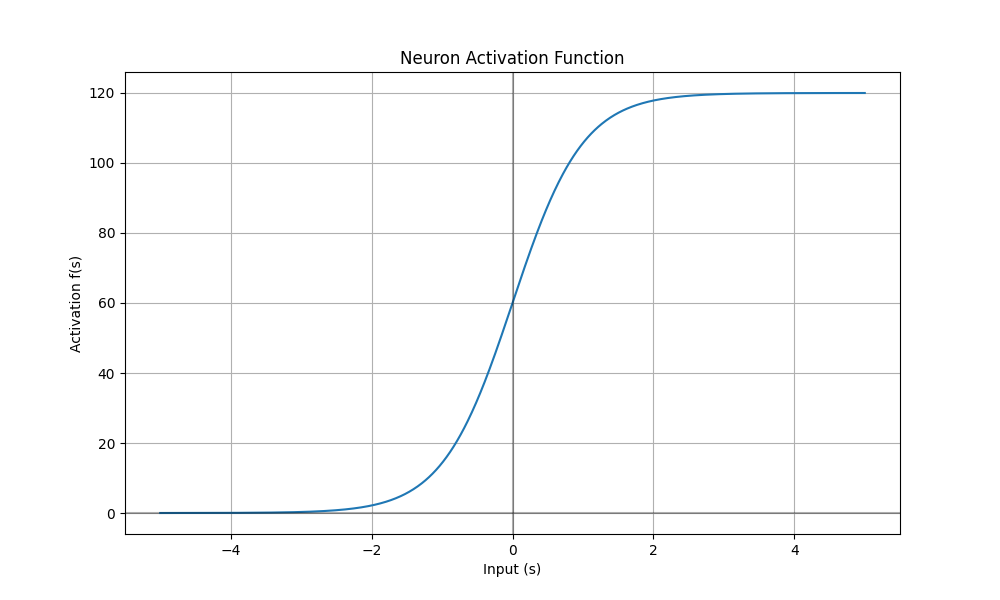
\includegraphics[width=0.8\textwidth]{activation_function.png}
    \caption{Plot of the activation function $f(s) = 60(1 + \tanh(s))$ over the input range $[-5, 5]$. The function shows the characteristic S-shape of a sigmoid, with output values ranging from 0 to 120 spikes per second.}
    \label{fig:activation}
\end{figure}

\subsection{Study the dynamics}

When simulating the system with three initial conditions $r(0) = 59$, $r(0) = 60$, and $r(0) = 61$, we observe interesting dynamical behavior:

\begin{itemize}
    \item For $r(0) = 59$: The firing rate decreases and settles at the lower stable fixed point.
    \item For $r(0) = 60$: The firing rate remains constant, indicating this is an unstable fixed point.
    \item For $r(0) = 61$: The firing rate increases and settles at the higher stable fixed point.
\end{itemize}

This behavior indicates the system has three fixed points, with the middle one ($r \approx 60$) acting as a threshold. Initial conditions below this threshold lead to a low firing rate state, while initial conditions above it lead to a high firing rate state. This is characteristic of a bistable system.

\begin{figure}[H]
    \centering
    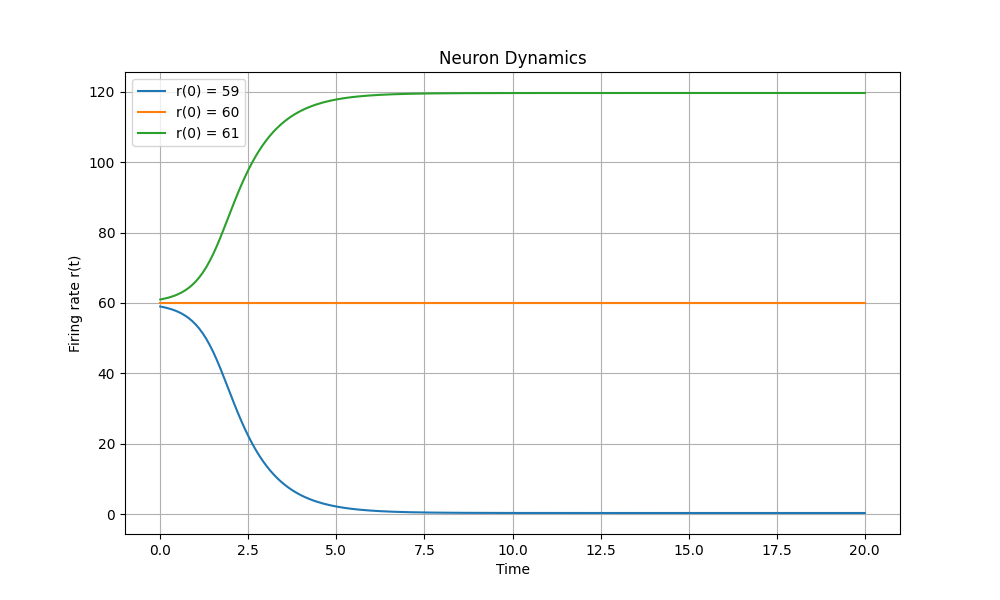
\includegraphics[width=0.8\textwidth]{deterministic_dynamics.png}
    \caption{Time evolution of the neuron firing rate $r(t)$ with three different initial conditions: $r(0) = 59$, $r(0) = 60$, and $r(0) = 61$. The trajectories demonstrate the bistable nature of the system, with two stable fixed points separated by an unstable threshold at $r \approx 60$.}
    \label{fig:deterministic}
\end{figure}

\subsection{Add noise - NOT FINAL}

Adding noise to the system reveals additional insights:

\begin{equation}
\frac{dr(t)}{dt} = -r(t) + f(wr(t) + I) + \sigma\eta(t)
\end{equation}

Where $\eta(t)$ is Gaussian white noise and $\sigma$ is the noise magnitude.

\begin{itemize}
    \item \textbf{(a)~Low noise} ($\sigma = 0.1$): The system mostly maintains its bistable behavior, exhibiting only small stochastic excursions around the two attracting fixed points.  A trajectory that starts near $r_0 \!\approx\! 60\,$Hz drifts away because this intermediate firing rate is an \emph{unstable} fixed point, so the rate does \emph{not} remain constant there. 
    \item \textbf{(b)~Medium noise} ($\sigma = 1.0$): Larger fluctuations occasionally push trajectories across the separatrix, so the neuron sometimes switches between low- and high-firing states.
    \item \textbf{(c)~High noise} ($\sigma = 5.0$): Noise dominates the dynamics; trajectories hop back and forth between the two attractors so frequently that the system effectively loses any memory of its initial condition.
\end{itemize}

This demonstrates how noise can induce transitions between stable states in a bistable system, with the frequency of transitions increasing with noise magnitude.

\begin{figure}[H]
    \centering
    \begin{subfigure}[b]{0.48\textwidth}
        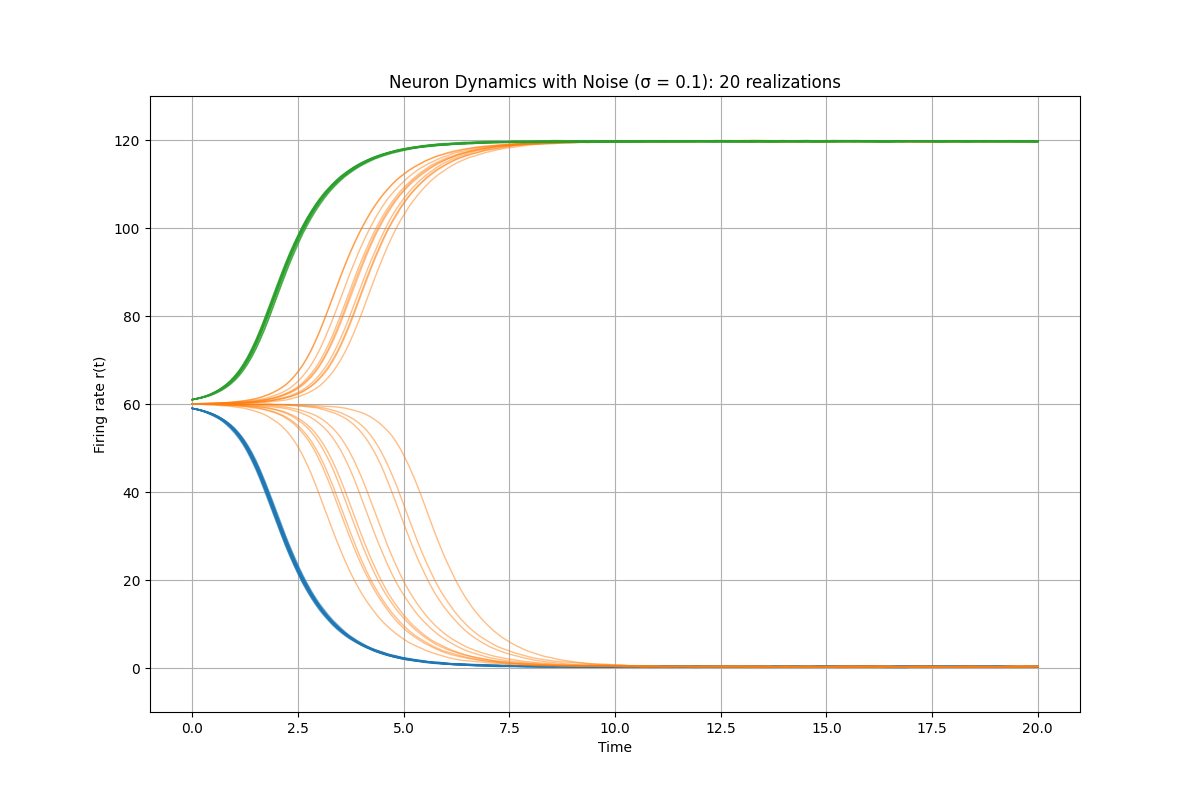
\includegraphics[width=\textwidth]{noise_strength_0.1.png}
        \caption{Low noise ($\sigma = 0.1$)}
        \label{fig:noise_low}
    \end{subfigure}
    \hfill
    \begin{subfigure}[b]{0.48\textwidth}
        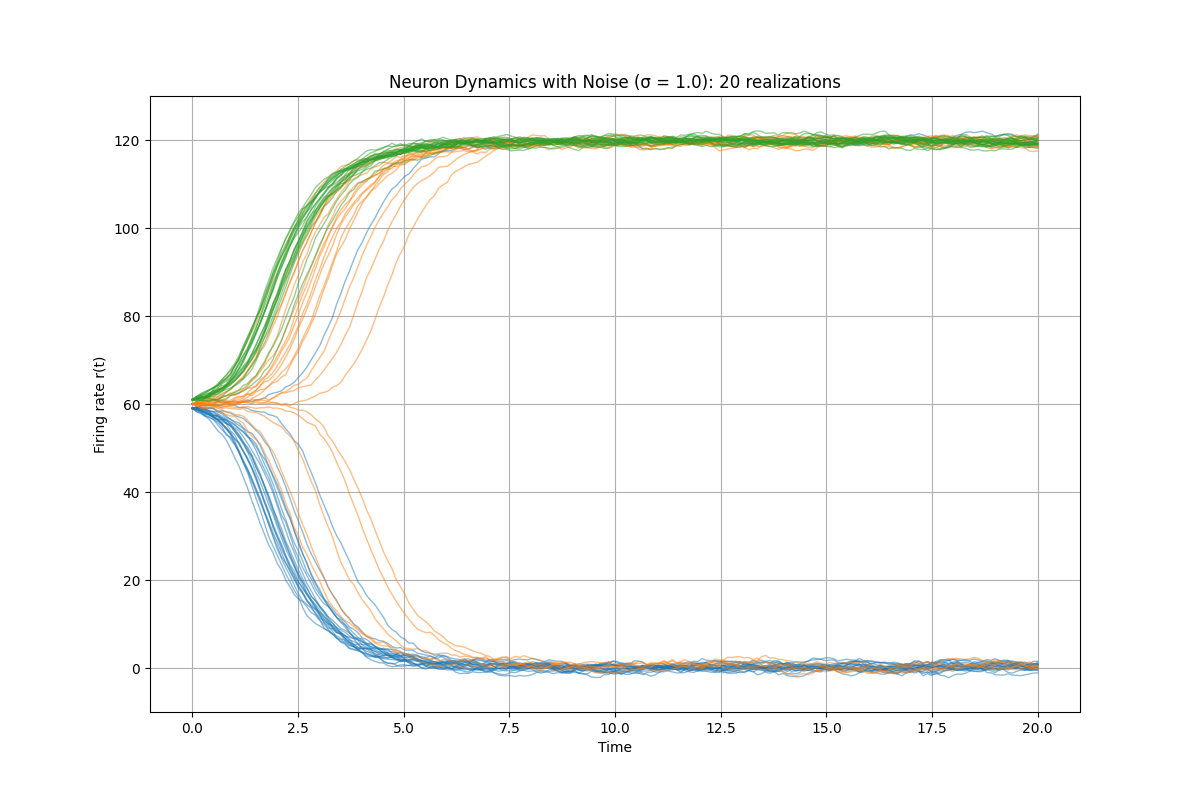
\includegraphics[width=\textwidth]{noise_strength_1.0.png}
        \caption{Medium noise ($\sigma = 1.0$)}
        \label{fig:noise_medium}
    \end{subfigure}
    
    \vspace{0.3cm}
    \begin{subfigure}[b]{0.48\textwidth}
        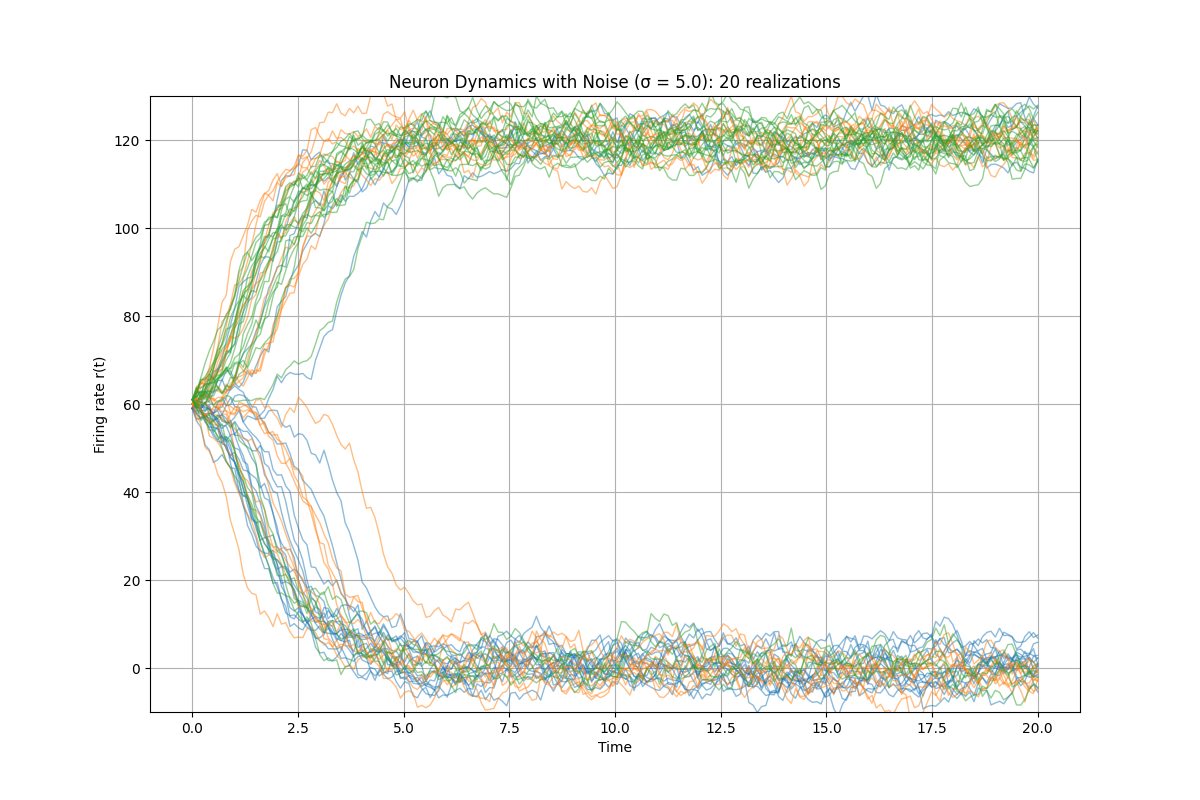
\includegraphics[width=\textwidth]{noise_strength_5.0.png}
        \caption{High noise ($\sigma = 5.0$)}
        \label{fig:noise_high}
    \end{subfigure}
    \caption{Effect of different noise levels on the neuron dynamics. As noise magnitude increases, transitions between stable states become more frequent, demonstrating how noise can induce state switching in a bistable system.}
    \label{fig:noise_effects}
\end{figure}


\subsection{Study the flux}


The flux analysis examines the derivative $\frac{dr}{dt}$ as a function of the firing rate $r$. The plot of this flux function reveals:

\begin{itemize}
    \item Three zero-crossings (fixed points) where $\frac{dr}{dt} = 0$:
    \begin{enumerate}
        \item Lower fixed point: Stable (negative slope at crossing)
        \item Middle fixed point: Unstable (positive slope at crossing)
        \item Upper fixed point: Stable (negative slope at crossing)
    \end{enumerate}
\end{itemize}

The stability of these fixed points can be determined by the slope of the flux function at each crossing:
\begin{itemize}
    \item Negative slope: Stable fixed point (perturbing the system slightly causes it to return to the fixed point)
    \item Positive slope: Unstable fixed point (perturbing the system slightly causes it to move away from the fixed point)
\end{itemize}

These findings confirm our observations from the time series simulations, providing a deeper understanding of the bistable nature of the system.

\begin{figure}[H]
    \centering
    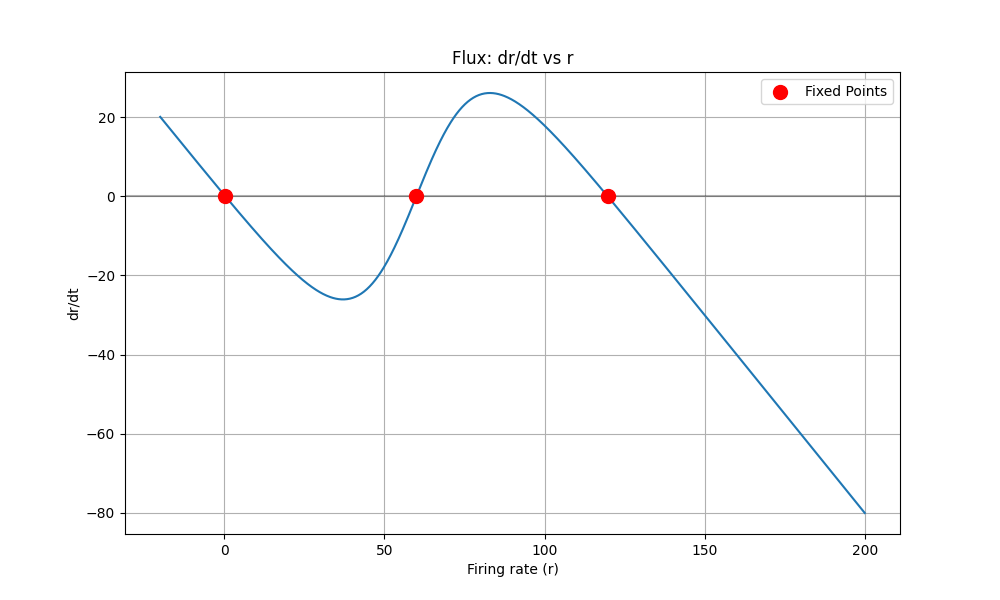
\includegraphics[width=0.8\textwidth]{flux_analysis.png}
    \caption{Flux analysis showing $\frac{dr}{dt}$ as a function of firing rate $r$. The zero-crossings represent fixed points of the system. The middle fixed point has a positive slope (unstable), while the other two have negative slopes (stable), confirming the bistable nature of the system.}
    \label{fig:flux}
\end{figure}


\subsection{Bifurcation diagram}

The bifurcation diagram explores how the number and nature of fixed points change as system parameters (synaptic strength $w$ and external input $I$) vary. The analysis reveals:

\begin{itemize}
    \item For low values of $w$ (weak self-connection): The system has a single stable fixed point.
    \item For intermediate values of $w$ and $I$: The system exhibits bistability with three fixed points (two stable, one unstable).
    \item For high values of $w$ (strong self-connection): The system can have more complex behavior.
\end{itemize}



\begin{figure}[H]
    \centering
    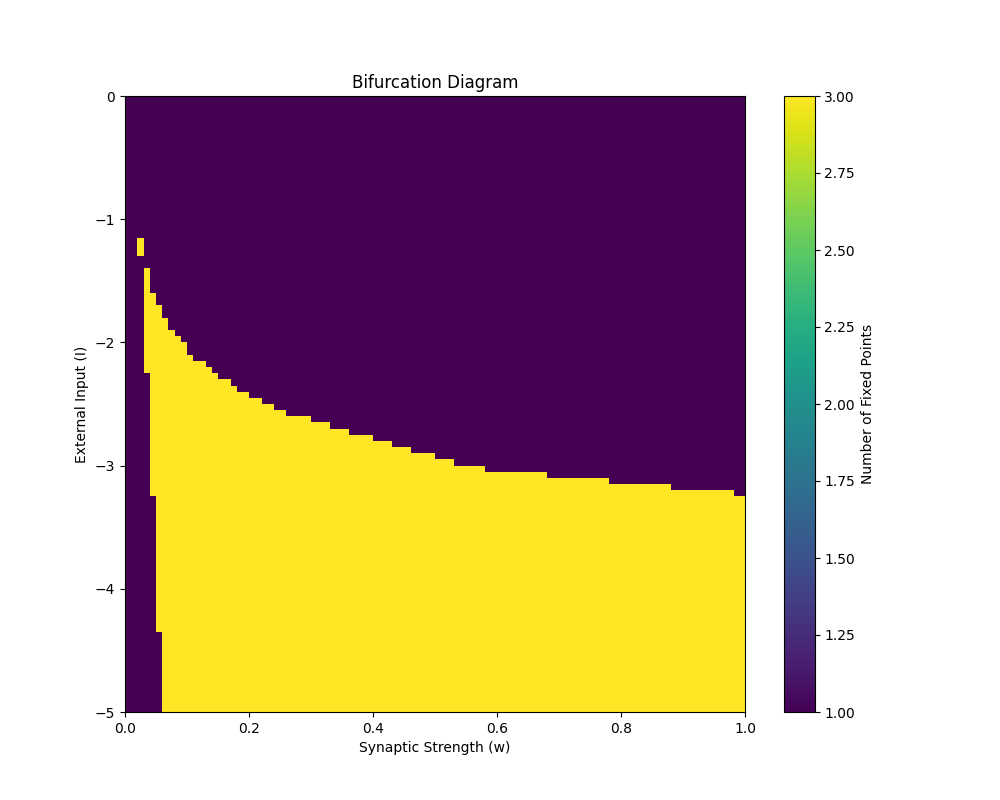
\includegraphics[width=0.6\textwidth]{bifurcation_diagram.png}
    \caption{Bifurcation diagram showing how the number of fixed points changes with synaptic strength ($w$) and external input ($I$). Different colors represent different numbers of fixed points. The boundaries between regions represent bifurcation points where the qualitative behavior of the system changes.}
    \label{fig:bifurcation}
\end{figure}




\section{Second Section}

% \subsection{First Subsection of Second Section}

% Description of analysis performed here.

% \begin{figure}[H]
% \centering
% \includegraphics[width=0.8\textwidth]{figure3.png}
% \caption{Figure caption}
% \label{fig:figure3}
% \end{figure}

% \begin{table}[H]
% \centering
% \begin{tabular}{lc}
% \toprule
% \textbf{Measure} & \textbf{Value} \\
% \midrule
% Measure 1    & Value 1 \\
% Measure 2    & Value 2 \\
% \bottomrule
% \end{tabular}
% \caption{Table caption}
% \label{tab:results}
% \end{table}

% Interpretation of results here.

\section{Conclusion}

Summary of main findings and their significance.

\end{document}
